%% ThreadLearn: Research Paper
%% Format: Springer LNCS (ICCIES 2026 compatible)
%% Based on template: ICCIES2026_256_NguyenThiThuyHoai.pdf

\documentclass[runningheads]{llncs}

%% ── Packages ────────────────────────────────────────────────────────────────
\usepackage[utf8]{inputenc}
\usepackage[T1]{fontenc}
\usepackage{booktabs}
\usepackage{multirow}
\usepackage{listings}
\usepackage{xcolor}
\usepackage{graphicx}
\usepackage[expansion=false]{microtype}
\usepackage{enumitem}
\usepackage{amssymb}
\usepackage{amsmath}
\usepackage[hidelinks]{hyperref}
\usepackage{url}
\usepackage{caption}
\usepackage{float}
\usepackage{tikz}
\usetikzlibrary{arrows, positioning, shapes, fit}
\usepackage{pgfplots}
\pgfplotsset{compat=1.16}


%% ── Code listing style ──────────────────────────────────────────────────────
\lstdefinestyle{codebase}{
  basicstyle=\small\ttfamily,
  keywordstyle=\color{blue!70!black}\bfseries,
  commentstyle=\color{gray!70},
  stringstyle=\color{green!50!black},
  numberstyle=\tiny\color{gray},
  numbers=left,
  numbersep=8pt,
  frame=single,
  framesep=4pt,
  breaklines=true,
  showstringspaces=false,
  tabsize=2,
  xleftmargin=12pt,
}
\lstdefinelanguage{JavaScript}{
  keywords={break,case,catch,continue,debugger,default,delete,do,else,
    finally,for,function,if,in,instanceof,new,return,switch,this,throw,
    try,typeof,var,let,const,void,while,with,async,await,class,of,from,
    import,export,extends,super,static,yield,Promise,require,module},
  sensitive=true,
  comment=[l]{//},
  morecomment=[s]{/*}{*/},
  morestring=[b]",
  morestring=[b]',
  morestring=[b]`,
}
\lstdefinestyle{js}{style=codebase, language=JavaScript}
\lstdefinestyle{py}{style=codebase, language=Python}

%% ════════════════════════════════════════════════════════════════════════════
\begin{document}

%% ── Title ───────────────────────────────────────────────────────────────────
\title{ThreadLearn: A RAG-Augmented Fine-Tuned Language Model\\
       for JavaScript Concurrency Bug Detection and Remediation}

\titlerunning{ThreadLearn: RAG-Augmented LLM for JS Concurrency Bugs}

\author{Le Tri Trung\inst{1}\orcidID{0009-0007-0790-1388} \and
        Ha Van An\inst{2}\orcidID{0009-0000-8536-4396} \and
        Nguyen Thi Thuy Hoai\inst{3}\orcidID{0009-0007-6328-0715}}

\authorrunning{L.T. Trung, H.V. An, and N.T.T. Hoai}

\institute{FPT University, Da Nang, Vietnam\\
  \email{letritrung2605@gmail.com}
\and
  FPT University, Da Nang, Vietnam\\
  \email{antruongkiet1412@gmail.com}
\and
  FPT University, Da Nang, Vietnam\\
  \email{hoaintt40@fe.edu.vn}}

\maketitle

%% ── Abstract ────────────────────────────────────────────────────────────────
\begin{abstract}
Concurrency bugs in asynchronous JavaScript (Node.js) code are a leading
cause of serious failures in production systems, including data races,
lost updates, and application hangs.
Existing tools fall into two categories: rule-based static detectors that
can identify suspicious patterns but cannot generate fixes, and large
language models (LLMs) that can reason about code but tend to miss the
exact buggy line and require large model sizes (7B--32B parameters) to
perform well.
ThreadLearn addresses both weaknesses by combining a 5-pattern static
race detector with a small language model (Qwen2.5-Coder-1.5B) fine-tuned
using QLoRA on 892 training examples with hindsight Chain-of-Thought
reasoning.
At inference time, a BM25 retrieval pipeline fetches the 3 most relevant
documents from a 2,050-document knowledge base to augment the prompt.
On a 30-case real-world benchmark drawn entirely from production npm packages
(rw\_01--rw\_30) spanning 10 concurrency bug categories, ThreadLearn with
the full BM25+AST pipeline achieves \textbf{22.0/30 (73.3\%)},
compared with 60.0\% for the base model without fine-tuning and 65.0\% for
GPT-3.5-turbo with the same pipeline---despite having $\sim$125$\times$
fewer parameters.
A key finding is that the retrieval pipeline only benefits models that
already have domain knowledge: the base model gains no benefit from retrieval
while the fine-tuned model gains $+$10 percentage points.
The fine-tuning dataset and evaluation scripts are publicly available.

\keywords{concurrency bugs \and race conditions \and static analysis \and
LLM fine-tuning \and retrieval-augmented generation \and JavaScript}
\end{abstract}

%% ════════════════════════════════════════════════════════════════════════════
\section{Introduction}
\label{sec:intro}

Asynchronous JavaScript (Node.js~\cite{nodejs}) is widely used for building
web backends, APIs, and real-time services, but the event-driven, non-blocking
execution model makes it easy to write code with subtle concurrency bugs.
A large-scale empirical study (NodeCB~\cite{nodecb2017}) analyzed 57 real
concurrency bugs across 53 open-source Node.js projects and found that
65\% involve atomicity violations, 30\% involve order violations, and
93\% cause serious consequences such as crashes, corrupted database state,
or process hangs.

Despite how common and harmful these bugs are, existing automated tools
still fall short.
Rule-based static analyzers (e.g., ESLint async rules, ThreadSanitizer)
can detect suspicious patterns but cannot explain or fix them, and they
generate false alarms on modern \texttt{async}/\texttt{await} code.
LLM-based approaches~\cite{pcwms2026} can reason about code semantics but
cannot pinpoint the exact buggy line without structural guidance, and they
require large models to achieve competitive accuracy.

We identify four concrete gaps in the state of the art:

\begin{description}[leftmargin=2em]
  \item[G1] Rule-based detectors find bugs but cannot generate fixes.
  \item[G2] LLM-only approaches ignore structural signals from
    static analysis and require 7B--32B parameter models.
  \item[G3] No existing tool uses static detector output as
    structured context to guide LLM reasoning.
  \item[G4] No end-to-end tool covers the full workflow of
    \emph{detect $\to$ explain $\to$ fix} for JavaScript (Node.js).
\end{description}

This paper makes four contributions:

\begin{enumerate}[leftmargin=2em]
  \item \textbf{\texttt{race\_detector}}: a 5-pattern static analyzer for
    JavaScript (Node.js) with an AST-based code preprocessor
    (\S\ref{sec:design:detector}).
  \item \textbf{Hindsight CoT dataset}: 892 training examples of the form
    \texttt{(code, detector\_output, reasoning\_trace, fix)}, where
    reasoning is written after the correct fix is known
    (\S\ref{sec:design:finetuning}).
  \item \textbf{ThreadLearn pipeline}: an end-to-end system that detects,
    retrieves context, and generates a fix, served via a FastAPI
    web endpoint (\S\ref{sec:design:arch}).
  \item \textbf{Evaluation}: comparison against a base LLM and GPT-3.5-turbo
    on a 30-case real-world JavaScript concurrency benchmark across fix pass
    rate, per-category accuracy, and ablation study (\S\ref{sec:eval}).
\end{enumerate}

Guided by the gaps above, we structure our evaluation around three research
questions:

\begin{description}[leftmargin=2.5em]
  \item[RQ1] Does combining a static race detector with a fine-tuned small
    language model outperform a general-purpose LLM (GPT-3.5-turbo) on
    real-world JavaScript concurrency bugs, despite having far fewer
    parameters? (answered in \S\ref{sec:eval:pipeline} and
    \S\ref{sec:eval:ablation})
  \item[RQ2] Does BM25+AST retrieval augmentation benefit every model
    equally, or does its benefit depend on whether the model has been
    fine-tuned on domain-specific data? (answered in
    \S\ref{sec:eval:nopipeline}--\S\ref{sec:eval:ablation})
  \item[RQ3] Which concurrency bug categories remain hard for a fine-tuned
    small model, and what does that reveal about the limits of pattern-based
    training data? (answered in \S\ref{sec:eval:category})
\end{description}

The remainder of the paper is organized as follows.
\S\ref{sec:background} introduces the Node.js concurrency bug taxonomy,
BM25 retrieval, and QLoRA fine-tuning that underpin our design.
\S\ref{sec:related} positions ThreadLearn against rule-based and
LLM-based prior work.
\S\ref{sec:design} describes the dataset, the static detector, the
hindsight Chain-of-Thought fine-tuning procedure, and the end-to-end
pipeline architecture.
\S\ref{sec:eval} reports experimental results, directly answering RQ1--RQ3.
\S\ref{sec:conclusion} summarizes findings and outlines future work.

%% ════════════════════════════════════════════════════════════════════════════
\section{Background}
\label{sec:background}

\paragraph{Concurrency bug taxonomy.}
Concurrency bugs in asynchronous JavaScript arise from the single-threaded
event loop model: a single thread interleaves callback execution, I/O
completion, and timer firing in an order that depends on runtime
scheduling rather than the order code is written.
Unlike race conditions in multi-threaded languages, which stem from
unsynchronized memory access across CPU cores, Node.js concurrency bugs
stem from \emph{interleaving} async operations whose relative completion
order is not guaranteed---two database writes issued back-to-back may
resolve in either order depending on network latency, queue depth, or
event-loop phase.
Table~\ref{tab:taxonomy} summarizes the four recurring bug types
identified in the NodeCB study~\cite{nodecb2017} and how each manifests
concretely in Node.js code.

\begin{table}[tb]
  \centering
  \caption{Concurrency bug types in Node.js (from NodeCB~\cite{nodecb2017}).}
  \label{tab:taxonomy}
  \begin{tabular}{@{}llp{5.5cm}@{}}
    \toprule
    \textbf{Bug Type} & \textbf{Rate} & \textbf{Manifestation in Node.js} \\
    \midrule
    Atomicity violation & 65\% & Two async operations overlap on shared state (e.g., lost database update) \\
    Order violation     & 30\% & Callback fires before dependent operation completes \\
    Starvation          & 5\%  & I/O queue exhausted; deferred tasks never execute \\
    Closure loop var    & JS   & \texttt{var i} shared by reference across all \texttt{setTimeout} callbacks \\
    \bottomrule
  \end{tabular}
\end{table}

Atomicity violations dominate (65\%) because Node.js encourages
fire-and-forget I/O: two logically atomic steps (e.g.\ check-then-update)
execute as separate, interruptible operations.
Order violations (30\%) occur when a callback assumes a prior async step
completed (e.g.\ reading a file before a preceding write flushed), and
starvation (5\%) is rarer but harder to diagnose since the hung-request
symptom appears far from its saturated-queue cause.
The fourth row, \emph{closure loop var}, is a JavaScript-specific pitfall
rather than a NodeCB category: function-scoped \texttt{var} makes a loop
variable referenced inside a deferred callback observe its \emph{final}
value rather than the value at scheduling time.
We include it because, though syntactic, it is among the most frequent
bugs in our benchmark (\S\ref{sec:design:dataset}) and is fully fixable by
a deterministic rewrite (\texttt{var}$\to$\texttt{let})---an ideal first
target for rule-based detection.

\paragraph{BM25 retrieval.}
BM25~\cite{bm25robertson} scores a document $D$ against query
$Q=\{q_1,\ldots,q_n\}$ by term frequency and inverse document frequency
with length normalization:
\[
  \text{BM25}(D, Q) = \sum_{i=1}^{n} \text{IDF}(q_i) \cdot
  \frac{f(q_i, D) \cdot (k_1 + 1)}{f(q_i, D) + k_1 \cdot (1 - b + b \cdot |D| / \overline{|D|})}
\]
with $k_1 = 1.5$, $b = 0.75$.
We use BM25 (via \texttt{rank-bm25}~\cite{rankbm25}) over dense vector
search because exact API name matching (e.g.\ \texttt{setTimeout}) is more
precise than semantic similarity for concurrency patterns.

\paragraph{QLoRA fine-tuning.}
QLoRA~\cite{qlora} fine-tunes a 4-bit NF4-quantized model via
LoRA~\cite{lora} adapters, updating only the adapter weights so training
fits on a single laptop GPU.
We use rank $r = 16$, scaling $\alpha = 32$.

%% ════════════════════════════════════════════════════════════════════════════
\section{Related Work}
\label{sec:related}

\emph{Rule-based detectors} match code against predefined patterns.
ThreadSanitizer~\cite{threadsanitizer} detects data races at runtime but
only on C/C++ and Java; ESLint~\cite{eslint} adds async rules for
JavaScript but only syntactic ones, missing semantic races across
callbacks; the NodeCB regex matcher~\cite{nodecb2017} has high
false-positive rates on modern \texttt{async}/\texttt{await} code; and
dynamic delay-injection (NACD~\cite{nacd2025}) exposes more event races but
still generates no fixes.
\emph{ML/LLM approaches} train on code features for defect detection, but
pre-trained code models are not concurrency-specific; PCWMs~\cite{pcwms2026}
applies reasoning world models to parallel code yet relies on 7B--32B
models and ignores static structure; and RAG code tools~\cite{rag_survey}
improve completion but have not been applied to JavaScript concurrency
remediation.
Table~\ref{tab:related} positions ThreadLearn against these tools along
four axes: detection, fix generation, JavaScript support, and fine-tuning.

\begin{table}[tb]
  \centering
  \caption{Comparison of ThreadLearn with related tools.}
  \label{tab:related}
  \begin{tabular}{@{}lcccc@{}}
    \toprule
    \textbf{Tool} & \textbf{Detect} & \textbf{Fix} & \textbf{JS} & \textbf{Fine-tuned} \\
    \midrule
    ThreadSanitizer      & $\checkmark$ & $\times$     & $\times$     & $\times$ \\
    ESLint async         & $\checkmark$ & $\times$     & $\checkmark$ & $\times$ \\
    NodeCB (rules)       & $\checkmark$ & $\times$     & $\checkmark$ & $\times$ \\
    PCWMs (LLM-only)     & $\checkmark$ & $\checkmark$ & $\checkmark$ & $\checkmark$ \\
    \textbf{ThreadLearn} & $\checkmark$ & $\checkmark$ & $\checkmark$ & $\checkmark$ \\
    \bottomrule
  \end{tabular}
\end{table}

The rule-based tools flag a line but leave the fix to the developer;
PCWMs generates fixes but without structural signal, so it must infer both
\emph{where} and \emph{how} from semantics alone (hence 7B--32B parameters).
ThreadLearn is the only entry combining all four axes: its detector narrows
the search to a specific \texttt{pattern\_id} and \texttt{line\_range}
before the LLM runs, letting a 1.5B model match a far larger
general-purpose model (\S\ref{sec:eval:ablation}).

%% ════════════════════════════════════════════════════════════════════════════
\section{Proposed Approach}
\label{sec:design}

\subsection{Dataset}
\label{sec:design:dataset}

Our study uses three datasets.
The \textbf{fine-tuning dataset} (892 examples) has the form
\texttt{(code, detector\_output, reasoning\_trace, fix)}, where each
reasoning trace is written by a teacher model \emph{after} the correct fix
is known (hindsight CoT), and was built entirely by the authors with no
crowdsourcing or model-generated labels.
It comprises 332 synthetic pairs (37.2\%)---handcrafted and manually
verified---and 560 generated pairs (62.8\%) produced by
\texttt{generate\_pairs()}, a template engine that expands the handcrafted
pairs over 40 domain slots (e.g.\ \texttt{User}, \texttt{Order}) using 18
generator functions, each a distinct concurrency transformation (e.g.\
sequential \texttt{await}$\to$\texttt{Promise.all}, callback$\to$\texttt{async},
unguarded \texttt{fetch}$\to$\texttt{AbortController} timeout).
Because each generator is a deterministic template, all generated labels
are correct by construction, avoiding the label noise of LLM-sampled data
while teaching the \emph{pattern} rather than specific names.

\textbf{Knowledge base.}
The retrieval knowledge base contains 2,050 JavaScript documents collected
from authoritative sources: MDN Web Docs~\cite{mdn} (99 documents covering
\texttt{Promise}, \texttt{async}/\texttt{await}, and Node.js API
behavior), official documentation of concurrency libraries
(RxJS, p-limit, async-mutex, Bluebird; 50 documents), curated ThreadLearn
pattern descriptions (151 documents), and 1,750 synthetic documents
generated via context permutation (re-phrasing API descriptions with
synonyms and varied identifiers) to broaden BM25 coverage of API name
variants.
All 2,050 documents fall into three groups: \texttt{patterns} (1,418),
\texttt{race-conditions} (352), and \texttt{anti-patterns} (280).

\textbf{Real-world evaluation benchmark.}
To avoid bias from self-generated test cases, we built a benchmark of 30
real-world JavaScript concurrency bugs drawn entirely from production
open-source packages.
Table~\ref{tab:benchmark} summarizes the distribution across 10 bug
categories.

\begin{table}[tb]
  \centering
  \vspace{-0.3cm}
  \caption{Real-world benchmark distribution (30 cases from production npm packages).}
  \label{tab:benchmark}
  \begin{tabular}{@{}lcc@{}}
    \toprule
    \textbf{Category} & \textbf{Count} & \textbf{Example Package} \\
    \midrule
    Race Condition      & 5  & \texttt{request}, \texttt{passport}, \texttt{bull} \\
    Double Callback     & 4  & \texttt{mysql}, \texttt{ioredis}, \texttt{async} \\
    Unhandled Rejection & 5  & \texttt{express}, \texttt{mongoose}, \texttt{co} \\
    Resource Exhaustion & 4  & \texttt{pg}, \texttt{axios}, \texttt{sequelize} \\
    Event Loop Blocking & 3  & \texttt{express} (sync middleware), Node.js crypto \\
    Sequential Awaits   & 3  & \texttt{express-session}, nodebestpractices~\cite{nodebestpractices} \\
    Zalgo               & 2  & \texttt{async} \\
    Context Loss        & 2  & \texttt{express-async-errors}, Node.js timers \\
    Stream Leak         & 1  & Node.js streams \\
    Callback Hell       & 1  & \texttt{async} \\
    \midrule
    \textbf{Total}      & \textbf{30} & \\
    \bottomrule
  \end{tabular}
\end{table}

Every case (rw\_01--rw\_30) traces to a specific GitHub issue or Node.js
API document (e.g.\ \texttt{request\#2484}, \texttt{mysqljs\#1260}), so no
case is synthetic; drawing them from independent production incidents
rather than the training-data engine eliminates model-favorable bias.
The full case-to-source list is in the public repository.

\subsection{Data Preprocessing and Evaluation Strategy}
\label{sec:design:preprocess}

\textbf{AST Preprocessing.}
ThreadLearn's preprocessor provides four esprima-based~\cite{esprima}
helpers shared by the detector and retrieval stage:
\texttt{stripComments} and \texttt{normalizeWhitespace} canonicalize the
source so the detector's regex patterns and BM25 query are not thrown off
by formatting; \texttt{extractFunctions} scopes detector line-ranges to a
function body; and \texttt{extract\_keywords} returns the top-20 identifier
names as the literal BM25 query---so preprocessing quality directly affects
retrieval precision.

\textbf{Evaluation strategy.}
Each test case specifies an expected fix pattern (e.g.\ \texttt{Promise.all},
\texttt{try/catch}, \texttt{let} in loop) and is scored \textbf{PASS} if
the generated code contains it, \textbf{PARTIAL} if code is generated
without the pattern, and \textbf{FAIL} if no code is generated.

\subsection{Model Architecture}
\label{sec:design:arch}

ThreadLearn has five independent modules that communicate through simple
data structures, allowing any module to be replaced independently.
Figure~\ref{fig:overview} shows the end-to-end pipeline, which follows
five sequential steps:

\begin{figure}[t]
  \centering
  \scriptsize
  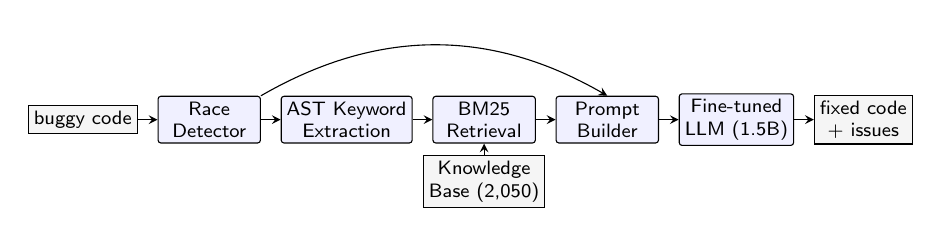
\begin{tikzpicture}[
    node distance=0.25cm and 0.25cm,
    box/.style={draw, rectangle, rounded corners=1pt,
                minimum width=1.3cm, minimum height=1.0em,
                font=\scriptsize\sffamily, align=center,
                inner sep=2pt, fill=blue!6},
    io/.style={draw, rectangle, rounded corners=0pt,
               minimum width=1.1cm, minimum height=1.0em,
               font=\scriptsize\sffamily, align=center,
               inner sep=2pt, fill=gray!8},
    arrow/.style={-stealth, thin},
  ]
    \node[io] (code) {buggy code};
    \node[box, right=of code] (det) {Race\\Detector};
    \draw[arrow] (code) -- (det);
    \node[box, right=of det] (ast) {AST Keyword\\Extraction};
    \draw[arrow] (det) -- (ast);
    \node[box, right=of ast] (bm25) {BM25\\Retrieval};
    \draw[arrow] (ast) -- (bm25);
    \node[io, below=0.15cm of bm25] (kb) {Knowledge\\Base (2,050)};
    \draw[arrow] (kb) -- (bm25);
    \node[box, right=of bm25] (prompt) {Prompt\\Builder};
    \draw[arrow] (bm25) -- (prompt);
    \draw[arrow] (det.north east) to[out=30, in=150] (prompt.north);
    \node[box, right=of prompt] (llm) {Fine-tuned\\LLM (1.5B)};
    \draw[arrow] (prompt) -- (llm);
    \node[io, right=of llm] (fix) {fixed code\\+ issues};
    \draw[arrow] (llm) -- (fix);
  \end{tikzpicture}
  \caption{ThreadLearn end-to-end pipeline. Buggy JavaScript code flows
           through five modules: static race detection, AST keyword extraction,
           BM25 retrieval from a 2,050-document knowledge base, prompt
           construction, and fine-tuned LLM inference to produce both
           a diagnosis and a corrected fix.}
  \label{fig:overview}
\end{figure}

The five steps are:
(1) \textbf{static detection}---\texttt{race\_detector} scans the source in
$O(n)$ time, emitting \texttt{\{pattern\_id, line\_range, description\}}
per match (\S\ref{sec:design:detector});
(2) \textbf{keyword extraction}---\texttt{extract\_keywords()} walks the
esprima AST and collects \texttt{Identifier} tokens as the BM25 query,
keeping CamelCase API names (e.g.\ \texttt{setTimeout}) intact rather than
splitting them;
(3) \textbf{retrieval}---BM25 returns the top-3 of 2,050 knowledge-base
documents;
(4) \textbf{prompt construction}---a \texttt{prompt\_builder} assembles the
detector report, retrieved documents, and buggy code into a structured
prompt;
(5) \textbf{fix generation}---the fine-tuned LLM outputs corrected code
with step-by-step reasoning.

\subsubsection{Static Race Detector.}
\label{sec:design:detector}

The detector checks 5 JavaScript concurrency patterns in two groups.
\emph{Closure/async}: \texttt{closure\_loop\_var} (\texttt{var} captured by
reference in loop callbacks), \texttt{shared\_var\_settimeout} (shared
variable modified inside \texttt{setTimeout}), and \texttt{promise\_no\_await}
(Promise created but not awaited).
\emph{Shared state}: \texttt{concurrent\_write\_array} (array mutated from
concurrent callbacks) and \texttt{counter\_no\_atomic} (non-atomic counter
increment).
For example, the \texttt{closure\_loop\_var} pattern fires when a
\texttt{var} loop variable is captured inside a \texttt{setTimeout} or
Promise callback, so all callbacks read the final loop value; the fix
replaces \texttt{var} with \texttt{let} to create a per-iteration binding.

\begin{lstlisting}[style=js, caption={\texttt{closure\_loop\_var}: bug (\texttt{var}, prints 5,5,...) vs.\ fix (\texttt{let}, prints 0,1,...).}]
for (var i = 0; i < 5; i++)             // bug:  always prints 5
  setTimeout(() => console.log(i), 100);
for (let i = 0; i < 5; i++)             // fix:  prints 0,1,2,3,4
  setTimeout(() => console.log(i), 100);
\end{lstlisting}

\subsubsection{Hindsight Chain-of-Thought Fine-Tuning.}
\label{sec:design:finetuning}

Training examples have the form:
\[
  (\textit{code},\; \textit{detector\_output},\; \textit{reasoning\_trace},\; \textit{fix})
\]
The \textit{reasoning\_trace} follows the Chain-of-Thought
paradigm~\cite{cot} but is written by a teacher model \emph{after} the
correct fix is known (hindsight reasoning), which yields a cleaner training
signal than forward reasoning under uncertainty.
We fine-tune Qwen2.5-Coder-1.5B~\cite{qwen25coder} with QLoRA ($r$=16,
$\alpha$=32, 4-bit NF4) via \texttt{SFTTrainer}~\cite{trl} on the 892
examples, grounding each on the detector's \texttt{pattern\_id} and
\texttt{line\_range}, on a single NVIDIA RTX 4060 laptop GPU.
This grounding---rather than raw code alone---is the key design choice: it
lets a 1.5B model learn a tractable mapping from a small, discrete set of
bug patterns to fixes instead of general concurrency reasoning from scratch.

%% ════════════════════════════════════════════════════════════════════════════
\section{Experimental Results and Discussions}
\label{sec:eval}

\label{sec:eval:setup}
\label{sec:eval:nopipeline}
\label{sec:eval:pipeline}
\label{sec:eval:ablation}

All experiments use the 30-case benchmark (\S\ref{sec:design:dataset}),
run on a Kaggle T4 GPU for local models and the OpenAI API for
GPT-3.5-turbo~\cite{gpt35}.
We evaluate six configurations---\{base, fine-tuned, GPT-3.5-turbo\}
$\times$ \{no-pipeline, +pipeline\}, where the pipeline is
AST keyword extraction $\to$ BM25 top-3 retrieval $\to$ augmented
prompt---scored PASS=1.0, PARTIAL=0.5, FAIL=0.
This staged design isolates the value of fine-tuning (models without
pipeline) from that of retrieval (each model with vs.\ without pipeline).

Table~\ref{tab:ablation} reports all six configurations.
Without any pipeline, the three models score within a narrow band
(60.0--63.3\%) with zero FAIL cases: every model emits syntactically valid
code, and the dominant failure mode is surface-level rewriting into
\texttt{async}/\texttt{await} syntax without addressing the underlying
hazard.
ThreadLearn merged already edges out GPT-3.5-turbo here ($+$0.5 pt),
confirming \textbf{G2}---without structural guidance even a strong
general-purpose LLM cannot reliably pinpoint the correct fix.
Adding the BM25+AST pipeline then separates the models sharply: the
fine-tuned model gains $+$3.0 pts ($+$10 pp), GPT-3.5-turbo gains only
$+$1.0 pt, and the base model gains \emph{nothing} (60.0\% in both
conditions) while introducing 2 FAIL cases.

\begin{table}[tb]
  \centering
  \vspace{-0.3cm}
  \caption{Full ablation on 30-case real-world benchmark (score = PASS + 0.5$\times$PARTIAL).}
  \label{tab:ablation}
  \begin{tabular}{@{}lccccc@{}}
    \toprule
    \textbf{Configuration} & \textbf{Pass} & \textbf{Partial} & \textbf{Fail}
      & \textbf{Score/30} & \textbf{\%} \\
    \midrule
    Base (no fine-tune, no pipeline)         & 6  & 24 & 0 & 18.0 & 60.0\% \\
    GPT-3.5-turbo (no pipeline)              & 7  & 23 & 0 & 18.5 & 61.7\% \\
    Fine-tuned only (no pipeline)            & 8  & 22 & 0 & 19.0 & 63.3\% \\
    Base + pipeline                          & 8  & 20 & 2 & 18.0 & 60.0\% \\
    GPT-3.5-turbo + pipeline                 & 9  & 21 & 0 & 19.5 & 65.0\% \\
    \textbf{ThreadLearn + pipeline} & \textbf{14} & \textbf{16}
      & \textbf{0} & \textbf{22.0} & \textbf{73.3\%} \\
    \midrule
    \multicolumn{4}{@{}l@{}}{\textit{Fine-tuning contribution (no pipeline):}}
      & $+$1.0 & $+$3.3\,pp \\
    \multicolumn{4}{@{}l@{}}{\textit{Pipeline contribution (fine-tuned model):}}
      & $+$3.0 & $+$10.0\,pp \\
    \multicolumn{4}{@{}l@{}}{\textit{Combined gain (ThreadLearn vs.\ base):}}
      & $+$4.0 & $+$13.3\,pp \\
    \bottomrule
  \end{tabular}
\end{table}

Three conclusions follow.
First, \textbf{fine-tuning is a prerequisite for pipeline benefit}: the
base model cannot use retrieved documentation constructively (0 pp, 2 new
FAILs).
Second, \textbf{the pipeline amplifies fine-tuning}---it adds $+$3.0 pts
on top of fine-tuning's $+$1.0 pt, a 3$\times$ larger gain.
Third, \textbf{ThreadLearn (73.3\%) beats GPT-3.5-turbo+pipeline (65.0\%)
by $+$2.5 pts despite $\sim$125$\times$ fewer parameters} (1.5B vs.\
$\sim$175B).

\textbf{Answering RQ1 and RQ2.}
The third conclusion answers \textbf{RQ1}: combining the static detector
with a fine-tuned 1.5B model outperforms GPT-3.5-turbo despite the
parameter disadvantage, because the detector's structured output narrows
what the LLM must infer.
The first answers \textbf{RQ2}: BM25+AST retrieval does \emph{not} benefit
every model equally---$+$10 pp for the fine-tuned model versus $0$ pp (and
regression) for the base model---so retrieval augmentation only pays off
once a model already has the domain knowledge to exploit it.

\subsection{Per-Category Analysis and RQ3}
\label{sec:eval:category}

Breaking the 22.0/30 score down by category, ThreadLearn is strongest on
Unhandled Rejection (90\%), Sequential Awaits (100\%), and Race Condition
(70\%, up from 50\% for both baselines)---categories well-represented in
training and tied to specific fix templates (\texttt{try}/\texttt{catch},
\texttt{Promise.all}, \texttt{var}$\to$\texttt{let}).
It is weakest on Zalgo, Double Callback, and Stream Leak (all 50\%), the
last being the only category where it trails the base model.
This answers \textbf{RQ3}: these categories remain hard because their
fixes require tracing \emph{callback invocation order} across asynchronous
boundaries---a semantic property not inferable from local syntactic
context---whereas our template-generated training data
(\S\ref{sec:design:dataset}) is dominated by syntactic substitutions.
Pattern-template data thus generalizes well to syntactically-fixable bugs
but underrepresents bugs needing multi-step temporal reasoning.

On latency, ThreadLearn ($\approx$26\,s/case) is $\sim$14$\times$ slower
than the GPT-3.5-turbo API ($\approx$1.8\,s) with $<$0.5\,s pipeline
overhead---a cost--privacy trade-off, since local inference runs on-device
at no per-call cost with no data leaving the machine.

%% ════════════════════════════════════════════════════════════════════════════
\section{Conclusion and Research Directions}
\label{sec:conclusion}

ThreadLearn addresses the gap between static detection and automated
remediation by combining a 5-pattern rule-based race detector with a small
language model (Qwen2.5-Coder-1.5B) fine-tuned on 892 hindsight
Chain-of-Thought examples and a BM25+AST retrieval pipeline.
On a 30-case real-world benchmark drawn entirely from production npm
packages, ThreadLearn achieves \textbf{22.0/30 (73.3\%)}---a $+$13.3 pp
gain over the base model and $+$8.3 pp over GPT-3.5-turbo with the same
pipeline, despite $\sim$125$\times$ fewer parameters.
It is the first end-to-end system to pair a rule-based race detector with
a fine-tuned small language model and RAG for JavaScript concurrency bug
remediation, bridging PCWMs~\cite{pcwms2026} (LLM-only, large model) and
rule-based detectors (ESLint, ThreadSanitizer) that produce no fixes.
The ablation establishes a design principle: \emph{retrieval only helps
models that already have domain knowledge}, so pipeline augmentation
should be paired with domain-specific fine-tuning rather than applied
standalone.

Future work will (1) expand the static detector to cover TypeScript AST
patterns; (2) add mutex and semaphore patterns for broader concurrency
coverage; and (3) investigate whether a larger fine-tuned model
(e.g., Qwen2.5-Coder-7B) would push Unhandled Rejection and Race Condition
above 75\%.

%% ════════════════════════════════════════════════════════════════════════════
\begin{thebibliography}{99}

\bibitem{nodecb2017}
  J.\ Wang, W.\ Dou, Y.\ Gao, C.\ Gao, F.\ Qin, K.\ Yin, and
  J.\ Wei.
  \newblock A Comprehensive Study on Real World Concurrency Bugs in
  {Node.js} ({NodeCB}).
  \newblock In \emph{Proc.\ 32nd IEEE/ACM ASE}, pp.\ 520--531, 2017.

\bibitem{pcwms2026}
  G.\ Singh, A.\ Guha, B.\ Kailkhura, and H.\ Menon.
  \newblock Learning Reasoning World Models for Parallel Code.
  \newblock \emph{arXiv:2604.20926}, 2026.

\bibitem{qlora}
  T.\ Dettmers, A.\ Pagnoni, A.\ Holtzman, and L.\ Zettlemoyer.
  \newblock {QLoRA}: Efficient Finetuning of Quantized LLMs.
  \newblock In \emph{Proc.\ NeurIPS}, 2023.

\bibitem{threadsanitizer}
  K.\ Serebryany and T.\ Iskhodzhanov.
  \newblock {ThreadSanitizer}: Data Race Detection in Practice.
  \newblock In \emph{Proc.\ WBIA}, pp.\ 62--71, 2009.

\bibitem{nacd2025}
  A.\ T.\ Endo and A.\ M{\o}ller.
  \newblock Event Race Detection for {Node.js} Using Delay Injections.
  \newblock In \emph{39th European Conference on Object-Oriented Programming (ECOOP 2025)}, pp.\ 9:1--9:28, 2025.

\bibitem{qwen25coder}
  Qwen Team.
  \newblock {Qwen2.5-Coder} Technical Report.
  \newblock \emph{arXiv:2409.12186}, 2024.

\bibitem{bm25robertson}
  S.\ Robertson and H.\ Zaragoza.
  \newblock The Probabilistic Relevance Framework: BM25 and Beyond.
  \newblock \emph{Foundations and Trends in Information Retrieval},
  vol.\ 3, no.\ 4, pp.\ 333--389, 2009.

\bibitem{rag_survey}
  P.\ Lewis, E.\ Perez, A.\ Piktus, et al.
  \newblock Retrieval-Augmented Generation for Knowledge-Intensive NLP Tasks.
  \newblock In \emph{Proc.\ NeurIPS}, 2020.

\bibitem{lora}
  E.\ J.\ Hu, Y.\ Shen, P.\ Wallis, et al.
  \newblock {LoRA}: Low-Rank Adaptation of Large Language Models.
  \newblock In \emph{Proc.\ ICLR}, 2022.

\bibitem{trl}
  L.\ von Werra, Y.\ Belkada, L.\ Tunstall, et al.
  \newblock {TRL}: Transformer Reinforcement Learning.
  \newblock \url{https://github.com/huggingface/trl}, 2020.

\bibitem{esprima}
  A.\ Hidayat.
  \newblock Esprima: ECMAScript Parsing Infrastructure.
  \newblock \url{https://esprima.org}, 2012.

\bibitem{eslint}
  N.\ C.\ Zakas.
  \newblock {ESLint}: The Pluggable JavaScript Linter.
  \newblock \url{https://eslint.org}, 2013.

\bibitem{nodejs}
  R.\ Dahl.
  \newblock {Node.js}: Evented I/O for V8 JavaScript.
  \newblock \url{https://nodejs.org}, 2009.

\bibitem{gpt35}
  OpenAI.
  \newblock {GPT-3.5 Turbo}.
  \newblock \url{https://platform.openai.com/docs/models/gpt-3-5-turbo}, 2023.

\bibitem{mdn}
  Mozilla.
  \newblock {MDN Web Docs}: JavaScript Reference.
  \newblock \url{https://developer.mozilla.org/en-US/docs/Web/JavaScript}, 2024.

\bibitem{nodebestpractices}
  Y.\ Goldberg et al.
  \newblock The {Node.js} Best Practices Repository.
  \newblock \url{https://github.com/goldbergyoni/nodebestpractices}, 2017.

\bibitem{cot}
  J.\ Wei, X.\ Wang, D.\ Schuurmans, et al.
  \newblock Chain-of-Thought Prompting Elicits Reasoning in Large Language Models.
  \newblock In \emph{Proc.\ NeurIPS}, 2022.

\bibitem{rankbm25}
  D.\ Brown.
  \newblock {rank-bm25}: A Collection of BM25 Algorithms in Python.
  \newblock \url{https://github.com/dorianbrown/rank_bm25}, 2020.

\end{thebibliography}

\end{document}
